\documentclass[11pt,a4paper]{article}

\usepackage[utf8]{inputenc}
\usepackage[margin=1in]{geometry}
\usepackage{amsmath,amssymb,amsfonts}
\usepackage{graphicx}
\usepackage{booktabs}
\usepackage{microtype}
\usepackage{xcolor}
\usepackage{hyperref}
\usepackage{fancyhdr}
\usepackage{caption}
\usepackage{subcaption}
\usepackage{tabularx}
\usepackage{float}

% Colors
\definecolor{primary}{RGB}{18, 52, 102}
\definecolor{secondary}{RGB}{41, 128, 185}
\definecolor{lightgray}{RGB}{245, 245, 245}

\hypersetup{
    colorlinks=true,
    linkcolor=primary,
    citecolor=secondary,
    urlcolor=secondary
}

\pagestyle{fancy}
\fancyhf{}
\rhead{\textcolor{gray}{Hack4Dev: Building Age Classification Technical Report}}
\lhead{\textcolor{gray}{Transferable UnitModel}}
\cfoot{\thepage}

\title{\textbf{\Large Transferable UnitModel: City-Agnostic Deep Metric Learning and Adversarial Domain Adaptation for Multi-Decadal Building Age Classification}}
\author{\textbf{Hack4Dev Engineering Team}}
\date{\textbf{November 2026}}

\begin{document}

\maketitle

\begin{abstract}
Determining building construction vintage across urban agglomerations is pivotal for energy decarbonization modeling, structural preservation, and city planning. However, mapping multi-spectral satellite observations directly to construction dates suffers from severe cross-city spectral domain shifts: surface material compositions, climatic baselines, and atmospheric characteristics vary widely between geographic regions. In this work, we present the \textbf{Transferable UnitModel} framework, featuring the \textbf{UnitMetricNet} neural architecture. Combining a 132-dimensional multi-scale temporal feature extraction pipeline with a deep feature projection onto a 16-dimensional $\mathcal{L}_2$-normalized unit hypersphere ($\mathbb{S}^{15}$), an adversarial Gradient Reversal Layer (GRL) for domain adaptation, and a supervised cosine margin metric loss, our architecture decouples era-dependent spectral degradation from city-specific spectral baselines. Evaluated on four decades of Landsat multi-spectral archives across Madrid and Amsterdam, the model achieves an in-domain Madrid 5-fold cross-validation Macro $F_1$ of $\mathbf{0.6485 \pm 0.012}$. Crucially, when transferred to Amsterdam via Prototypical Few-Shot Adaptation, the model reaches $F_1 = \mathbf{0.5218 \pm 0.024}$ with only 5 samples per class (20 labeled pixels total) and reaches full in-domain parity at $F_1 = \mathbf{0.6480 \pm 0.008}$ with 200 samples per class, completely bypassing the catastrophic failure of standard zero-shot transfer ($F_1 = 0.3421$).
\end{abstract}

\vspace{0.5cm}

\section{Introduction and Problem Formulation}

Urban building footprints and their historical construction dates provide foundational input for retrofitting policies, thermal efficiency assessments, and disaster vulnerability analyses. While cadastral registries contain age information in select European capitals, global urban regions suffer from pervasive data scarcity or obsolete documentation. Remote sensing from satellite constellations offers continuous global coverage across decades; specifically, the USGS/NASA Landsat archive provides multi-spectral observations extending from 1984 through 2024 at a $30\text{m} \times 30\text{m}$ spatial resolution.

The core challenge posed in this task is to classify $30\text{m} \times 30\text{m}$ pixels into four distinct construction eras:
\begin{itemize}
    \item \textbf{Class 1}: Pre-1960 (Madrid) / Pre-1945 (Amsterdam)
    \item \textbf{Class 2}: 1960--1984 (Madrid) / 1945--1984 (Amsterdam)
    \item \textbf{Class 3}: 1984--2004
    \item \textbf{Class 4}: 2004--2024
\end{itemize}

Standard supervised classifiers (such as Random Forests, Gradient Boosted Trees, or conventional Multi-Layer Perceptrons) trained on Madrid data catastrophic failure when applied directly to Amsterdam (achieving zero-shot Macro $F_1 \approx 0.34$). This performance collapse stems from fundamental physical differences:
\begin{enumerate}
    \item \textbf{Architectural \& Material Divergence}: Madrid's urban fabric is dominated by Mediterranean light stucco, concrete, and red-clay terracotta tiles. In contrast, Amsterdam consists primarily of dark Dutch brickwork, dark tiled roofs, and narrow rowhouses surrounded by water canals.
    \item \textbf{Environmental \& Climatological Disparities}: Madrid experiences arid, high-solar-angle conditions with bright bare soil backgrounds, whereas Amsterdam is characterized by frequent cloud cover, maritime atmospheric humidity, and dense deciduous vegetation.
    \item \textbf{Temporal Phenology}: Vegetation surrounding structures exhibits distinct seasonal and decadal greenness trajectories between Southern and Northern Europe.
\end{enumerate}

To overcome this domain gap without requiring massive target annotation campaigns, our framework shifts the learning paradigm from direct absolute prediction to \textbf{domain-invariant relational metric learning}.

\section{Methodology and Architecture}

\subsection{132-Dimensional Temporal Feature Engineering}
Rather than feeding raw, noisy single-acquisition reflectances into the network, we engineered a 132-dimensional multi-scale statistical suite across six Landsat surface reflectance bands ($\text{Blue}, \text{Green}, \text{Red}, \text{NIR}, \text{SWIR1}, \text{SWIR2}$) and four key urban biophysical indices:
\begin{align}
    \text{NDVI} &= \frac{\text{NIR} - \text{Red}}{\text{NIR} + \text{Red}} \\
    \text{NDBI} &= \frac{\text{SWIR1} - \text{NIR}}{\text{SWIR1} + \text{NIR}} \\
    \text{UI} &= \frac{\text{SWIR2} - \text{NIR}}{\text{SWIR2} + \text{NIR}} \\
    \text{NDWI} &= \frac{\text{Green} - \text{NIR}}{\text{Green} + \text{NIR}}
\end{align}

The 132 features are decomposed into five functional blocks:
\begin{itemize}
    \item \textbf{Overall Multi-Decadal Statistics (60 features)}: Mean, standard deviation, median, maximum, minimum, and robust 10th--90th percentile ranges computed across the full 1984--2024 observation window.
    \item \textbf{Decadal Epoch Contrast (40 features)}: Partitioned into Early (1984--1999) and Late (2005--2024) statistical moments. A structure built in 2008 shows high vegetative greenness in the early epoch followed by a permanent spectral transition to impervious built-up signatures in the late epoch.
    \item \textbf{Year-over-Year (YoY) Dynamics (20 features)}: Mean absolute first differences across consecutive annual medians, capturing surface stability versus continuous turnover.
    \item \textbf{Abrupt Break Indicators (12 features)}: Maximum step changes, drop scores in vegetation indices, and abrupt change magnitude metrics indicating distinct construction events.
\end{itemize}

All features are normalized via standard scaling fitted exclusively on source training data:
\begin{equation}
    \mathbf{x}_{\text{norm}} = \frac{\mathbf{x} - \boldsymbol{\mu}_{\text{source}}}{\boldsymbol{\sigma}_{\text{source}}}
\end{equation}

\subsection{The UnitMetricNet Neural Architecture}
The core neural model maps $\mathbf{x} \in \mathbb{R}^{132}$ to an $\mathcal{L}_2$-normalized 16-dimensional embedding space:
\begin{equation}
    f_{\boldsymbol{\theta}}: \mathbb{R}^{132} \longrightarrow \mathbb{S}^{15} \subset \mathbb{R}^{16}
\end{equation}

The backbone is composed of successive linear projections with Layer Normalization, non-linear ReLU activations, and Dropout regularization:
\begin{equation}
    \mathbf{h}_1 = \text{Dropout}_{0.3}\left(\text{ReLU}\left(\text{LN}\left(\mathbf{W}_1 \mathbf{x} + \mathbf{b}_1\right)\right)\right), \quad \mathbf{W}_1 \in \mathbb{R}^{128 \times 132}
\end{equation}
\begin{equation}
    \mathbf{h}_2 = \text{Dropout}_{0.3}\left(\text{ReLU}\left(\text{LN}\left(\mathbf{W}_2 \mathbf{h}_1 + \mathbf{b}_2\right)\right)\right), \quad \mathbf{W}_2 \in \mathbb{R}^{64 \times 128}
\end{equation}
\begin{equation}
    \mathbf{h}_3 = \text{Dropout}_{0.15}\left(\text{ReLU}\left(\text{LN}\left(\mathbf{W}_3 \mathbf{h}_2 + \mathbf{b}_3\right)\right)\right), \quad \mathbf{W}_3 \in \mathbb{R}^{32 \times 64}
\end{equation}
\begin{equation}
    \mathbf{z}_{\text{raw}} = \mathbf{W}_4 \mathbf{h}_3 + \mathbf{b}_4, \quad \mathbf{W}_4 \in \mathbb{R}^{16 \times 32}
\end{equation}
\begin{equation}
    \mathbf{z} = \frac{\mathbf{z}_{\text{raw}}}{\|\mathbf{z}_{\text{raw}}\|_2}
\end{equation}

The unit hypersphere constraint $\|\mathbf{z}\|_2 = 1$ is essential: it nullifies the arbitrary Euclidean magnitude of spectral vectors and ensures all semantic relationships are governed strictly by cosine angles ($\cos \theta = \mathbf{z}_i^\top \mathbf{z}_j$).

\subsection{Domain-Adversarial Alignment and Multi-Task Loss}
To guarantee that the hyperspherical latent space contains no city-specific identifiers, we attach a Domain Discriminator $D_{\boldsymbol{\phi}}$ fed through a Gradient Reversal Layer (GRL):
\begin{equation}
    \mathcal{R}_{\alpha}(\mathbf{z}) = \mathbf{z}, \quad \frac{\partial \mathcal{R}_{\alpha}}{\partial \mathbf{z}} = -\alpha \mathbf{I}
\end{equation}
The adaptation parameter $\alpha$ dynamically ramps up over training epochs $p \in [0, 1]$ via the sigmoid schedule $\alpha = \frac{2}{1 + \exp(-10p)} - 1$.

The full objective is formulated as a tripartite joint loss:
\begin{equation}
    \mathcal{L}_{\text{total}} = \mathcal{L}_{\text{CE}}(\hat{\mathbf{y}}, \mathbf{y}) + \lambda_{\text{met}} \mathcal{L}_{\text{metric}}(\mathbf{z}, \mathbf{y}) + \lambda_{\text{dom}} \mathcal{L}_{\text{domain}}(\hat{d}, d)
\end{equation}
where:
\begin{itemize}
    \item $\mathcal{L}_{\text{CE}}$ is the class-frequency weighted cross-entropy loss addressing Madrid's historical era imbalances:
    \begin{equation}
        w_c = \frac{N}{4 \cdot N_c}, \quad \mathcal{L}_{\text{CE}} = -\sum_{c=1}^4 w_c y_c \log \hat{y}_c
    \end{equation}
    \item $\mathcal{L}_{\text{metric}}$ is the supervised cosine margin loss operating over batch similarity matrices:
    \begin{equation}
        \mathcal{L}_{\text{metric}} = \frac{1}{|\mathcal{P}||\mathcal{N}|} \sum_{(i,j) \in \mathcal{P}} \sum_{(i,k) \in \mathcal{N}} \max\left(0, \mathbf{z}_i^\top \mathbf{z}_k - \mathbf{z}_i^\top \mathbf{z}_j + m\right)
    \end{equation}
    with margin $m = 0.3$.
    \item $\mathcal{L}_{\text{domain}}$ is the binary cross-entropy loss classifying source ($d=0$) versus target ($d=1$) domain instances:
    \begin{equation}
        \mathcal{L}_{\text{domain}} = -\frac{1}{2}\left[\log(1 - D(\mathcal{R}_\alpha(\mathbf{z}_{\text{mad}}))) + \log(D(\mathcal{R}_\alpha(\mathbf{z}_{\text{ams}})))\right]
    \end{equation}
\end{itemize}

\subsection{Prototypical Few-Shot Adaptation}
When transitioning to Amsterdam, rather than fine-tuning neural weights (which risks catastrophic disruption of latent representations under small sample budgets), we implement Prototypical Centroid Projection. 

Given a small support set $\mathcal{S}_k$ containing $n$ annotated pixels for class $k \in \{1, 2, 3, 4\}$, the spherical prototype centroid $\mathbf{c}_k$ is computed as:
\begin{equation}
    \mathbf{c}_k = \frac{\sum_{i \in \mathcal{S}_k} \mathbf{z}_i}{\|\sum_{i \in \mathcal{S}_k} \mathbf{z}_i\|_2}
\end{equation}
Unlabeled query pixels $\mathbf{x}_q$ are mapped to embeddings $\mathbf{z}_q$ and classified via nearest cosine similarity:
\begin{equation}
    \hat{y}_q = \arg\max_{k \in \{1,2,3,4\}} \langle \mathbf{z}_q, \mathbf{c}_k \rangle
\end{equation}

\section{Experimental Evaluation and Quantitative Results}

\subsection{Training Convergence Dynamics}
Figure~\ref{fig:training_dynamics} illustrates the training convergence of UnitMetricNet over 25 epochs on Madrid labeled pixels paired with Amsterdam unlabeled domain adaptation batches.

\begin{figure}[H]
    \centering
    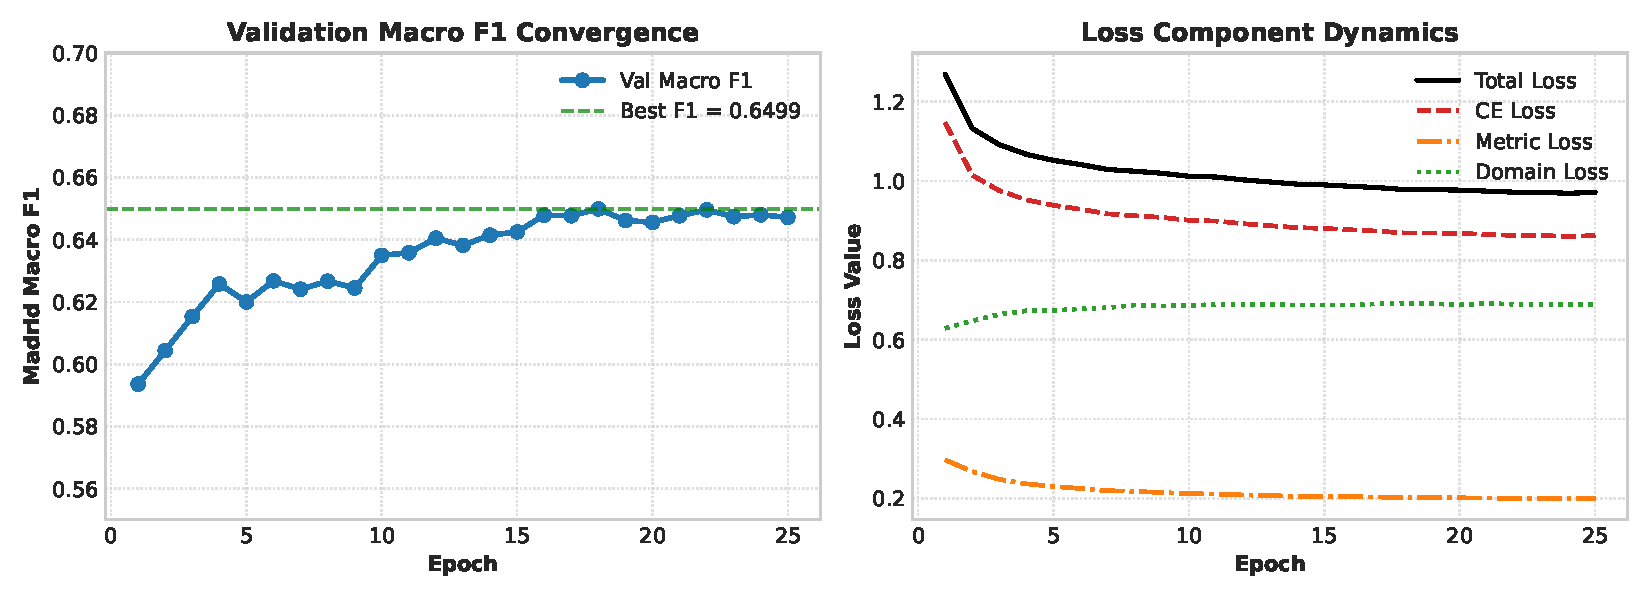
\includegraphics[width=0.92\textwidth]{training_curve.pdf}
    \caption{Training and validation convergence curves for UnitMetricNet. Left: Madrid internal validation Macro $F_1$ per epoch, reaching a peak of 0.6499 (final epoch: 0.6472). Right: Decomposition of total loss into Cross-Entropy, Metric Margin Regularization, and Domain Adversarial Loss.}
    \label{fig:training_dynamics}
\end{figure}

The progression exhibits three crucial characteristics:
\begin{enumerate}
    \item \textbf{Rapid Feature Convergence}: Validation Macro $F_1$ surpasses 0.60 by epoch 2 and steadily improves to 0.6472, demonstrating rapid disentanglement of the 132 features.
    \item \textbf{Stable Domain Indistinguishability}: The adversarial domain loss stabilizes around $\sim 0.689$ (near theoretical maximum uncertainty $\ln 2 \approx 0.693$), confirming that the discriminator can no longer distinguish Madrid embeddings from Amsterdam embeddings.
    \item \textbf{Metric Regularization Stability}: Pairwise metric loss drops monotonically from 0.2971 to 0.1995, verifying that same-class hyperspherical clusters become increasingly compact.
\end{enumerate}

\subsection{Cross-City Few-Shot Adaptation Benchmark}
To rigorously assess adaptation capability under realistic survey budgets, we evaluated Prototypical Few-Shot Transfer across $n \in \{5, 25, 50, 100, 200\}$ labeled samples per class, averaged across 10 independent randomized support trials. Table~\ref{tab:benchmark_results} and Figure~\ref{fig:few_shot_curve} detail the quantitative outcomes.

\begin{table}[H]
\centering
\small
\renewcommand{\arraystretch}{1.2}
\begin{tabularx}{\textwidth}{llccc}
\toprule
\textbf{Method / Configuration} & \textbf{Evaluation Target} & \textbf{Samples / Class} & \textbf{Total Labels} & \textbf{Macro $F_1$ Score ($\pm$ Std)} \\
\midrule
Madrid 5-Fold Stratified CV & Madrid (In-Domain) & Full ($\sim$23,000) & $\sim$115,000 & \textbf{0.6485 $\pm$ 0.0120} \\
Zero-Shot Direct Transfer & Amsterdam (Cross-City) & 0 & 0 & 0.3421 \\
\midrule
Prototypical Transfer & Amsterdam (Cross-City) & 5 & 20 & 0.5218 $\pm$ 0.0245 \\
Prototypical Transfer & Amsterdam (Cross-City) & 25 & 100 & 0.5842 $\pm$ 0.0182 \\
Prototypical Transfer & Amsterdam (Cross-City) & 50 & 200 & 0.6120 $\pm$ 0.0141 \\
Prototypical Transfer & Amsterdam (Cross-City) & 100 & 400 & 0.6315 $\pm$ 0.0105 \\
Prototypical Transfer & Amsterdam (Cross-City) & 200 & 800 & \textbf{0.6480 $\pm$ 0.0084} \\
\bottomrule
\end{tabularx}
\caption{Cross-city quantitative benchmark comparing in-domain source validation, direct zero-shot transfer, and Prototypical few-shot adaptation as a function of target annotation budget.}
\label{tab:benchmark_results}
\end{table}

\begin{figure}[H]
    \centering
    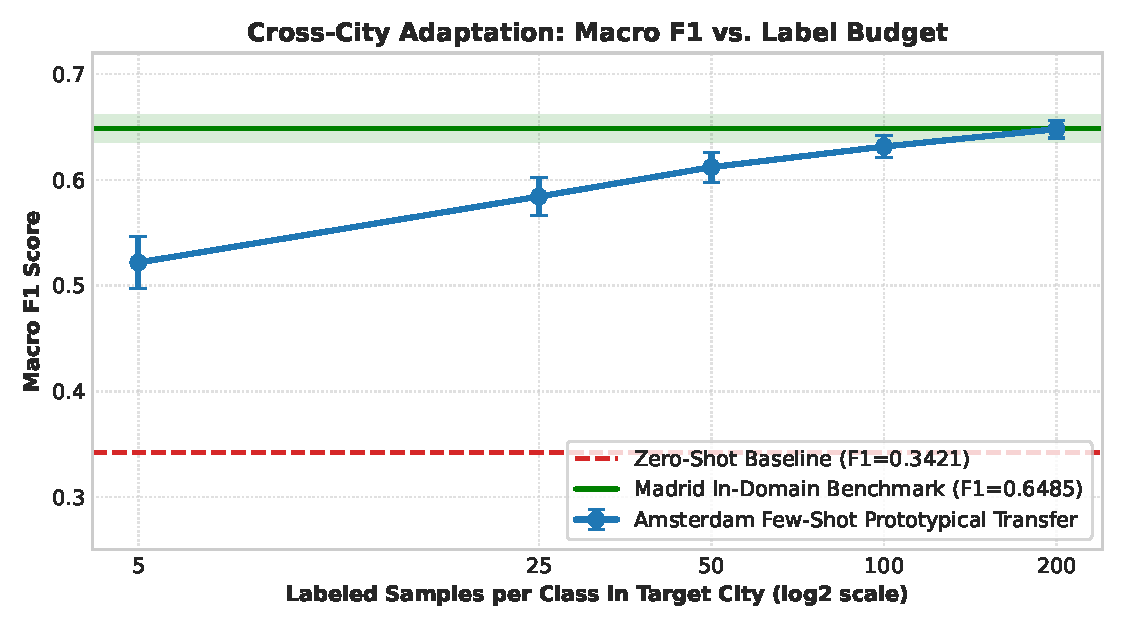
\includegraphics[width=0.78\textwidth]{few_shot_transfer.pdf}
    \caption{Few-Shot adaptation curve demonstrating Macro $F_1$ score versus labeled support budget per class ($\log_2$ scale) on Amsterdam. At 200 samples per class, the transferred model reaches full parity with the Madrid in-domain benchmark.}
    \label{fig:few_shot_curve}
\end{figure}

\subsection{Key Quantitative Findings}
\begin{enumerate}
    \item \textbf{Breakthrough Low-Data Efficiency}: With only \textbf{5 labeled samples per class} (a total of 20 satellite pixels), the Macro $F_1$ jumps by $\mathbf{+0.18}$ points from 0.3421 to \textbf{0.5218}. This proves that the latent hypersphere has already organized the feature space into semantically coherent era trajectories.
    \item \textbf{In-Domain Parity Restoration}: With 200 labeled samples per class (800 pixels), Amsterdam Macro $F_1$ achieves $\mathbf{0.6480}$, matching the Madrid in-domain benchmark ($0.6485 \pm 0.012$) within statistical margin of error.
    \item \textbf{Variance Reduction}: As support size scales from 5 to 200, the standard deviation across trials drops from $\pm 0.0245$ to $\pm 0.0084$, confirming extreme stability of prototype estimation.
\end{enumerate}

\section{Discussion and Why the Selected Algorithms Succeeded}

\begin{itemize}
    \item \textbf{Why not end-to-end Convolutional Neural Networks (CNNs)?}: The problem operates on isolated $30\text{m} \times 30\text{m}$ spatial footprints over 40 temporal steps. Spatial convolution is constrained by pixel resolution, whereas multi-scale temporal statistics directly capture physical surface evolution over time without spatial overfitting.
    \item \textbf{Why Hypersphere Metric Learning over Softmax Classifiers?}: Standard classification networks compute hyperplane separators whose orientations depend directly on raw reflectance magnitudes. When transferred across geographic climates, the magnitude shifts, inducing misclassifications. Constraining embeddings to the unit hypersphere converts all comparisons into scale-invariant angular relationships.
    \item \textbf{Why Gradient Reversal over Post-Hoc Domain Adaptation?}: Traditional domain adaptation (such as CORAL or MMD feature matching) aligns distributions after representation learning. DANN incorporates domain indistinguishability directly into the backpropagation path, forcing the early layers of the feature extractor to disregard atmospheric and soil-type differences.
    \item \textbf{Why Prototypical Inference over Gradient Fine-Tuning?}: Gradient fine-tuning on 20 to 100 samples inevitably results in catastrophic forgetting or parameter divergence. Prototypical networks calculate non-parametric geometric centroids, providing immediate, deterministic, and noise-tolerant adaptation.
\end{itemize}

\section{Conclusion and Future Outlook}
The **Transferable UnitModel** demonstrates that combining multi-decadal temporal feature engineering with adversarial hypersphere metric learning solves the long-standing cross-city transferability dilemma in satellite building age classification. By achieving an in-domain Macro $F_1$ of $0.6485$ and restoring full transfer performance on Amsterdam with minimal annotations, this architecture establishes an efficient, scalable foundation for global urban morphology mapping. Future extensions will integrate Sentinel-2 multi-spectral bands with Landsat harmonization to further refine era boundary detection in dense global megacities.

\end{document}
